\hypertarget{experiments}{
}

In the experimental stage of this research, two experiments are performed on two different datasets to analyse the overall quality of the synthesized data. The experiments conducted by Targhi for diffuse material classes are replicated and extended with synthesis using other reflection models, and the same setup is used on a new selection of material classes from the {\it PhoTex} database. The new selection of material classes have more glossy/shiny properties unlike the classes selected by Targhi, which should give a better indication for the quality of specularity simulated by Phong, Blinn-Phong and Torrance-Sparrow reflectance. 

\section{Preprocessing}\label{sec:preprocessing}
The {\it PhoTex} database consists of images recorded under a fixed point of view with varying light-source directions registered for each image. For the experiments, two datasets are chosen: a dataset according to the selection made by Targhi and another dataset with shiny properties to extend the experiments for the specular reflection models. 

The diffuse materials have the size After rendering new images for the materials and before extracting the features from the materials, the rendered images are set to zero-mean and unit-variance in order to make the features intensity-invariant. Since the diffuse and glossy/shiny materials have different image sizes, all images are cropped with respect to the center of the image to $200 \times 200$ pixels.

\subsection{Diffuse material classes}
Since we are interested in reproducing some results from the experiments of Targhi, and measure performance of more complex reflection models with respect to the Lambertian reflection model he applied, we need to select the same material classes he used in his experiment. These material classes are shown in figure \ref{fig:PhoTexData}.

From each material class, 40 images with certain slant and tilt angles are selected. The selected slant angles are $\{30^0, 45^0,60^0,75^0\}$. The images under a slant of $30^0$ have four different tilts, $\{0^0, 90^0, 180^0, 270^0\}$. The images with slants $\{45^0,60^0,75^0\}$ have tilts of $\{0^0,30^0,60^0,..., 300^0,330^0\}$. 

%\begin{comment}
\begin{figure}[h]
	\begin{center}
		\subfigure[aaa]{
\epsfig{file=images/db/aaa.eps, width=0.15\linewidth}}
		\subfigure[aab]{
\epsfig{file=images/db/aab.eps, width=0.15\linewidth}}
		\subfigure[aaj]{
\epsfig{file=images/db/aaj.eps, width=0.15\linewidth}}
		\subfigure[aam]{
\epsfig{file=images/db/aam.eps, width=0.15\linewidth}}
		\subfigure[aan]{
\epsfig{file=images/db/aan.eps, width=0.15\linewidth}}

		\subfigure[aao]{
\epsfig{file=images/db/aao.eps, width=0.15\linewidth}}
		\subfigure[aar]{
\epsfig{file=images/db/aar.eps, width=0.15\linewidth}}
		\subfigure[aas]{
\epsfig{file=images/db/aas.eps, width=0.15\linewidth}}
		\subfigure[aba]{
\epsfig{file=images/db/aba.eps, width=0.15\linewidth}}
		\subfigure[abj]{
\epsfig{file=images/db/abj.eps, width=0.15\linewidth}}

		\subfigure[abk]{
\epsfig{file=images/db/abk.eps, width=0.15\linewidth}}
		\subfigure[acc]{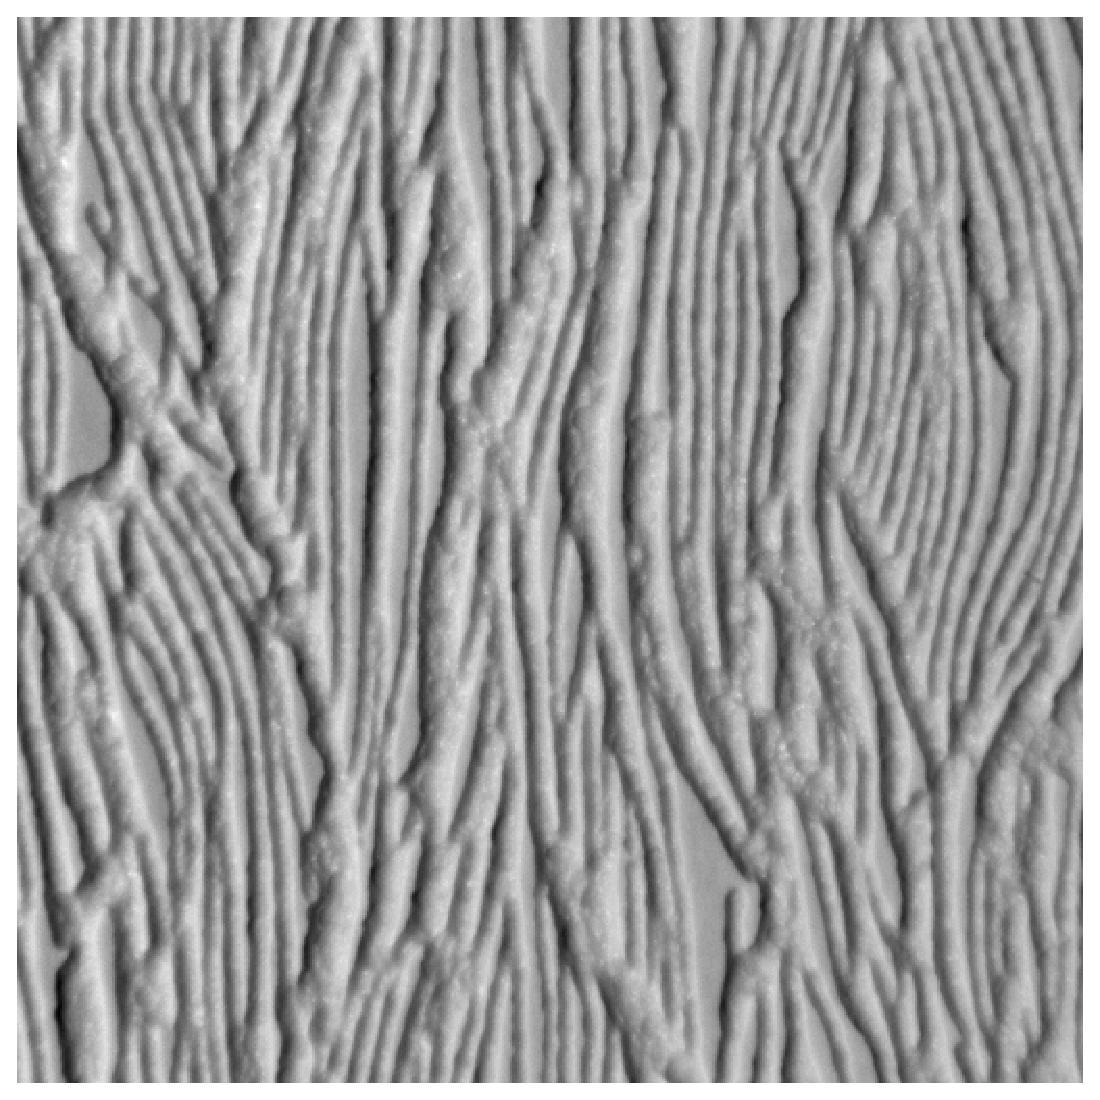
\epsfig{file=images/db/acc.eps, width=0.15\linewidth}}
		\subfigure[acd]{
\epsfig{file=images/db/acd.eps, width=0.15\linewidth}}
		\subfigure[ace]{
\epsfig{file=images/db/ace.eps, width=0.15\linewidth}}
		\subfigure[adb]{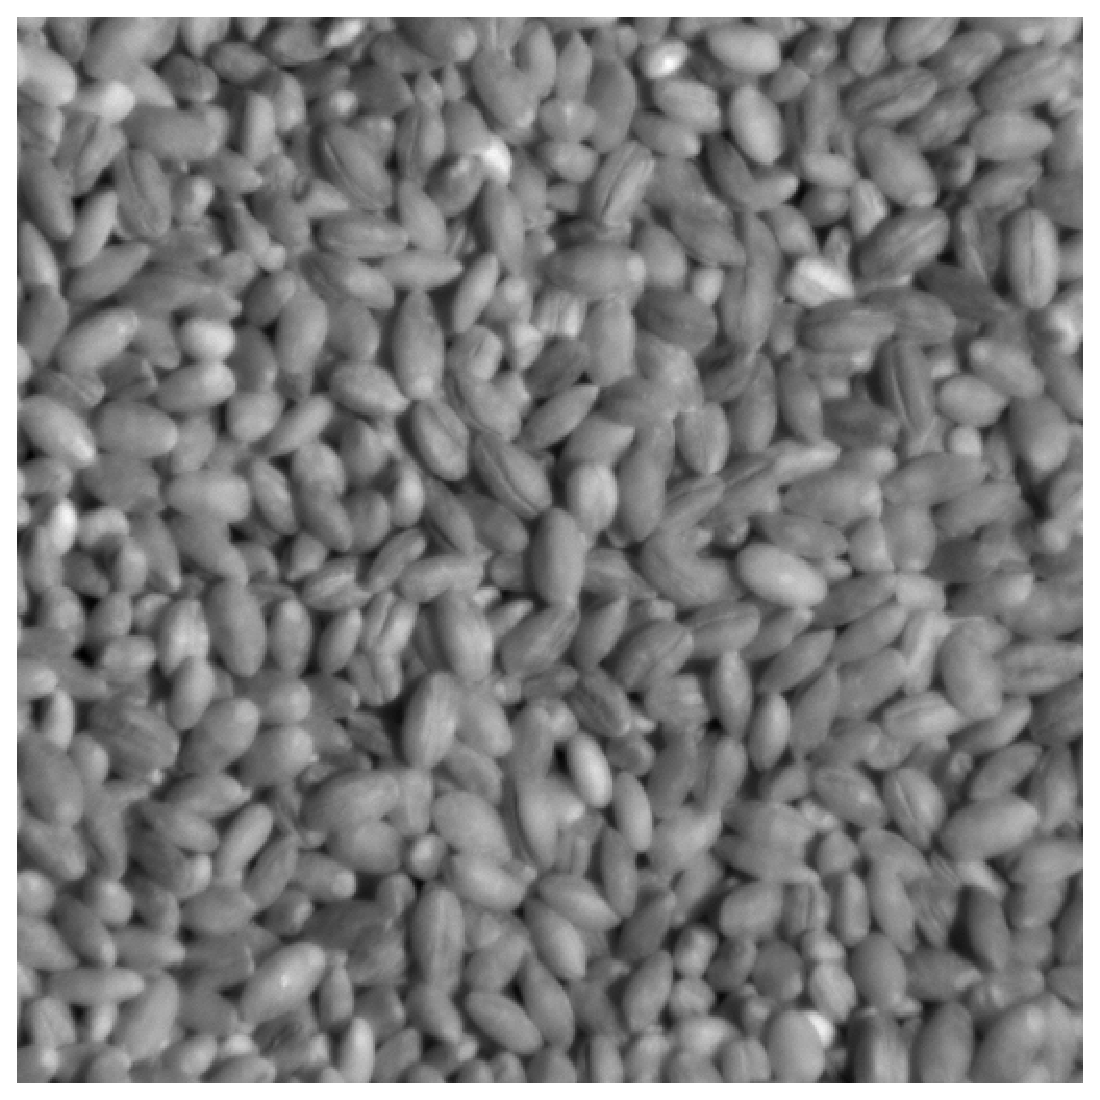
\epsfig{file=images/db/adb.eps, width=0.15\linewidth}}

		\subfigure[adc]{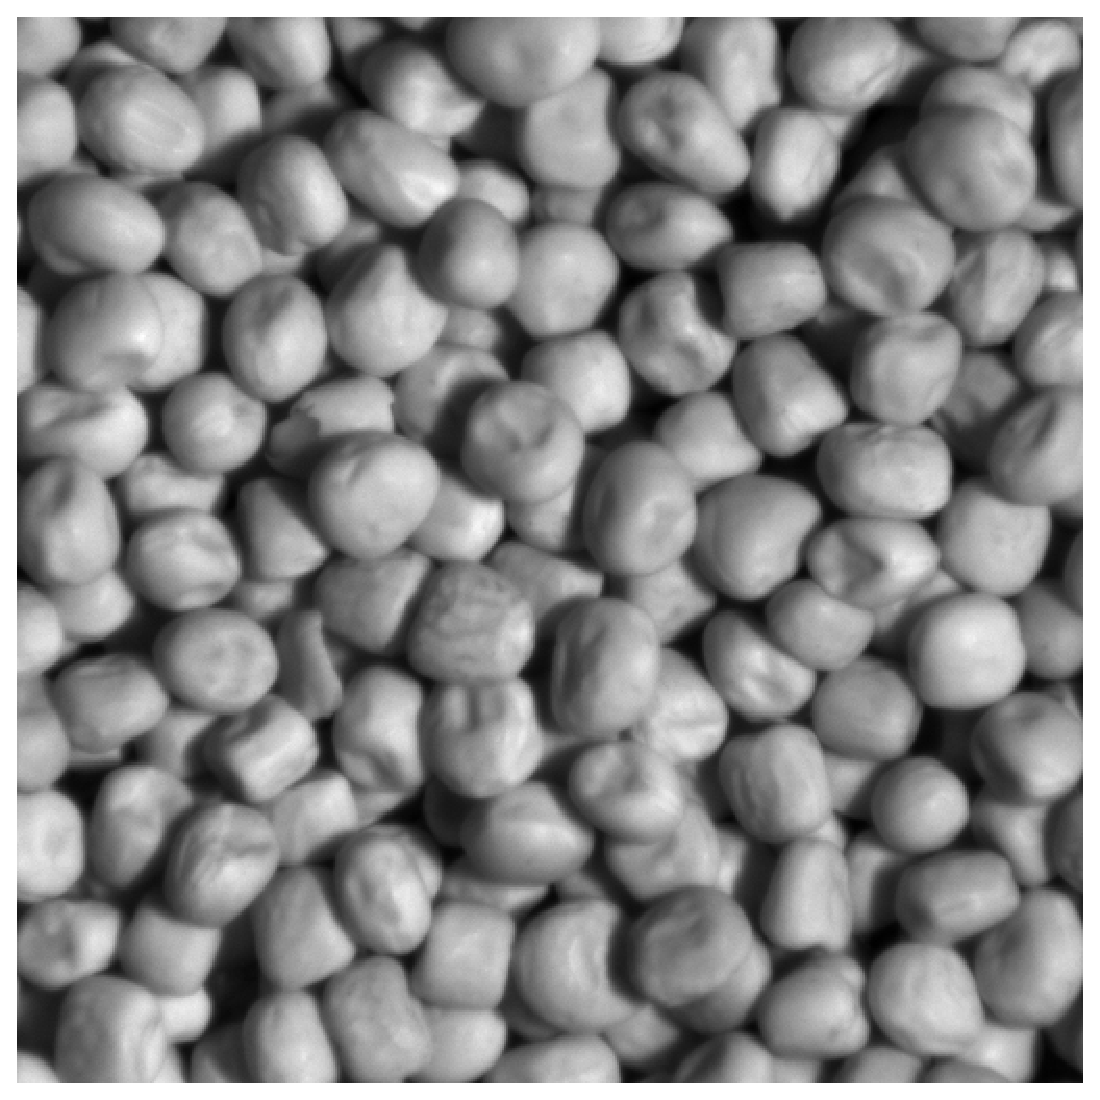
\epsfig{file=images/db/adc.eps, width=0.15\linewidth}}
		\subfigure[add]{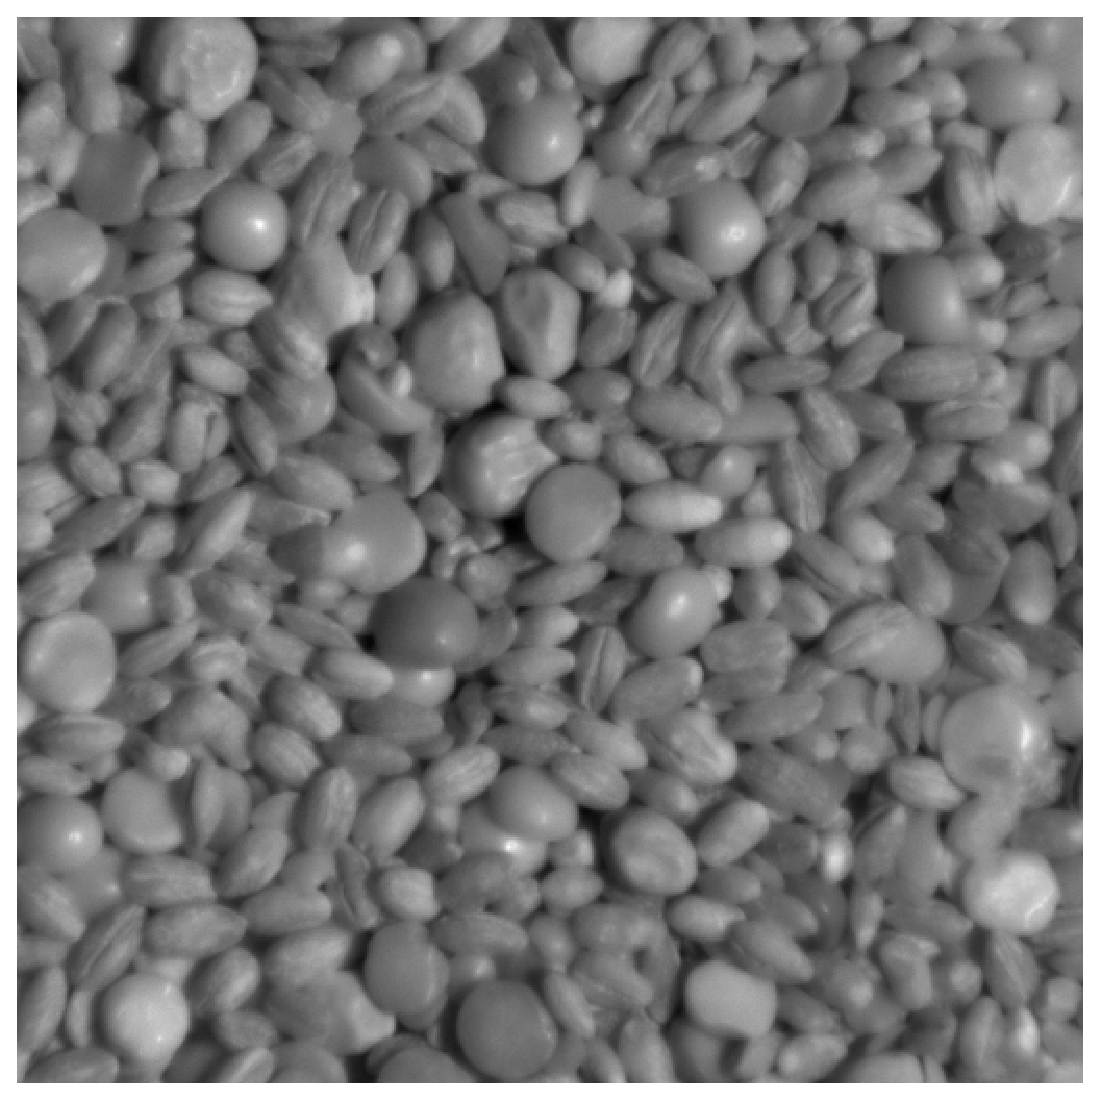
\epsfig{file=images/db/add.eps, width=0.15\linewidth}}
		\subfigure[ade]{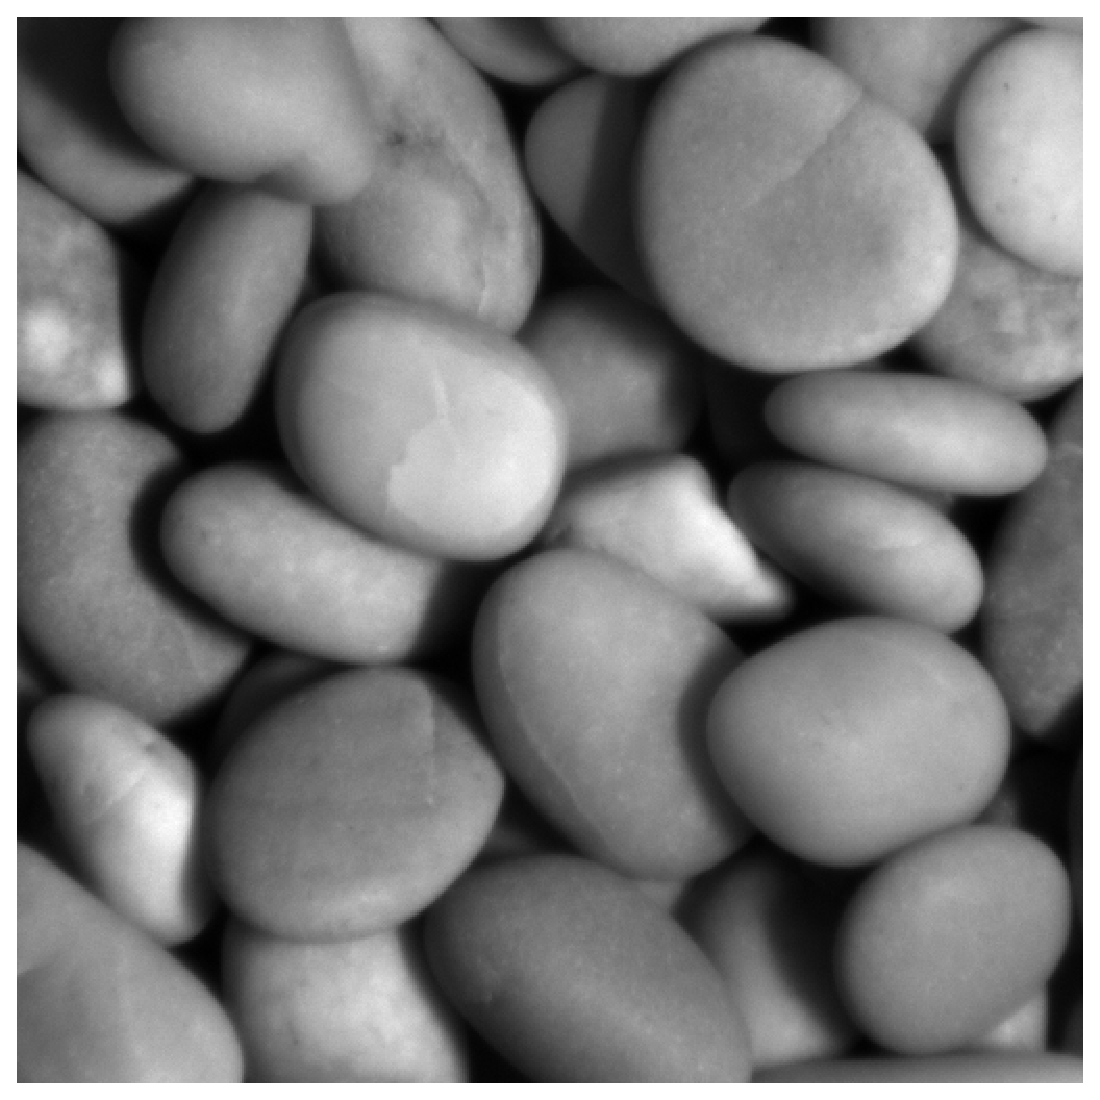
\epsfig{file=images/db/ade.eps, width=0.15\linewidth}}
		\subfigure[adg]{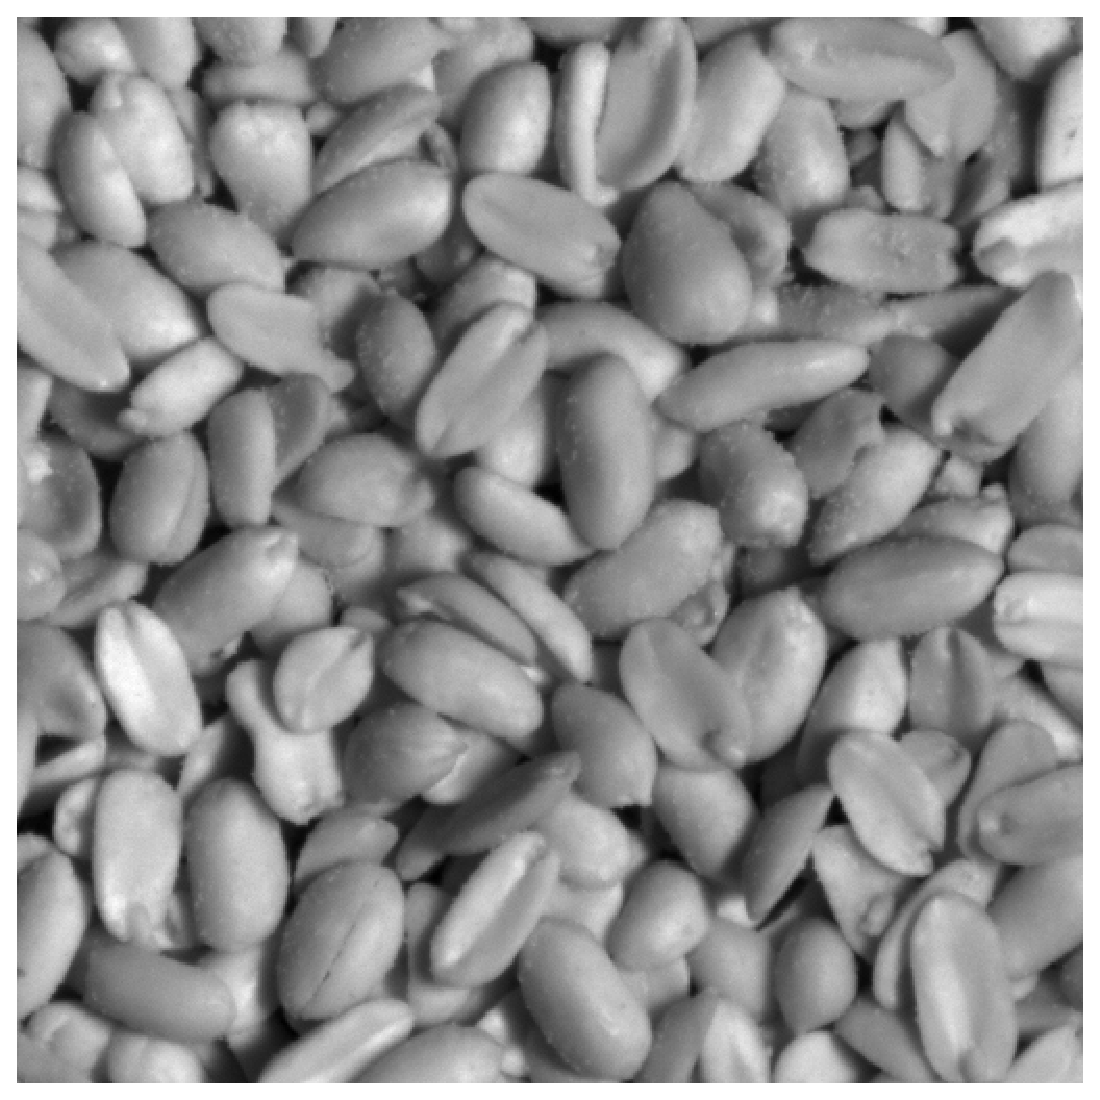
\epsfig{file=images/db/adg.eps, width=0.15\linewidth}}
		\subfigure[adh]{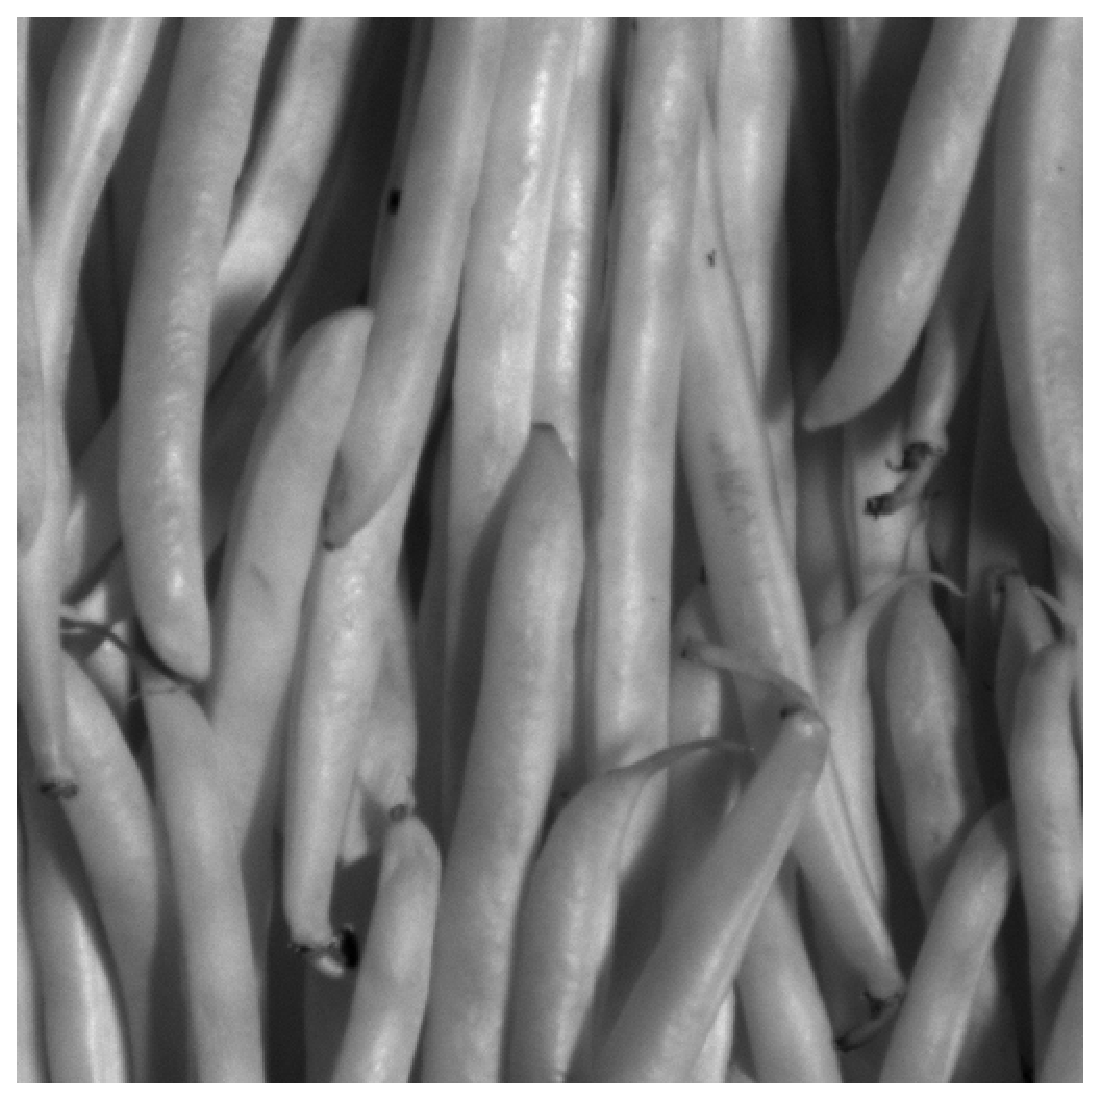
\epsfig{file=images/db/adh.eps, width=0.15\linewidth}}
	\end{center}
	\caption{{\it The material classes taken from the PhoTex database. The example images are registered under a slant of $30^0$ and a tilt of $0^0$.}}
	\label{fig:PhoTexData}
\end{figure}
%\end{comment}

\subsection{Shiny material classes}
Because three out of five reflection models simulate specularity only, the previous dataset might not be good enough to measure improvements made by these reflection models. For this reason, a new dataset is selected from the {\it PhoTex} database with more specular properties. 

The material classes selected are shown in figure X. This dataset consists of 10 material classes, recorded under a slant of $75^0$ and tilts of $0^0$ to $350^0$ in increments of $10^0$, giving a total of 36 images for each material class. The material classes are shown in figure \ref{fig:PhoTexData2}.

%\begin{comment}
\begin{figure}[h]
	\begin{center}
		\subfigure[aaa]{
\epsfig{file=images/db/aaa.eps, width=0.15\linewidth}}
		\subfigure[aab]{
\epsfig{file=images/db/aab.eps, width=0.15\linewidth}}
		\subfigure[aaj]{
\epsfig{file=images/db/aaj.eps, width=0.15\linewidth}}
		\subfigure[aam]{
\epsfig{file=images/db/aam.eps, width=0.15\linewidth}}
		\subfigure[aan]{
\epsfig{file=images/db/aan.eps, width=0.15\linewidth}}

		\subfigure[aao]{
\epsfig{file=images/db/aao.eps, width=0.15\linewidth}}
		\subfigure[aar]{
\epsfig{file=images/db/aar.eps, width=0.15\linewidth}}
		\subfigure[aas]{
\epsfig{file=images/db/aas.eps, width=0.15\linewidth}}
		\subfigure[aba]{
\epsfig{file=images/db/aba.eps, width=0.15\linewidth}}
		\subfigure[abj]{
\epsfig{file=images/db/abj.eps, width=0.15\linewidth}}
	\end{center}
	\caption{{\it The material classes taken from the PhoTex database. The example images are registered under a slant of $30^0$ and a tilt of $0^0$.}}
	\label{fig:PhoTexData2}
\end{figure}
%\end{comment}

\section{Reflection model parameters}\label{sec:ParameterSetting}
The reflection models used in the process of synthesis need material dependent parameters to be set, such as the parameter for the specular lobe size or surface roughness. However, these parameters are not available for the materials in the database in case of the micro-facet models, and in case of the empirical models there are no known 'good' values for the parameters to be set. To set these values, the parameters are computed using a gradient descent procedure with a total sum of squares error estimation:

		\begin{eqnarray*}
			Err(A,A') = \sum_{i=1}^n (a_i - a_i')^2
		\end{eqnarray*}
 
Where $A$ is the original image from the {\it PhoTex} database, and $A'$ is the synthesized image. By calculating the squared error per-pixel from the original image and the synthesized image, and accumulate the error over all pixels, an estimation of the total error serves as an indicator for the gradient descend. Both images are preprocessed to have zero-mean and unit-variance before the error is calculated, since the features will be extracted from preprocessed images.

Because the number of materials and the number of parameters to be estimated for each reflection model turn out to be large in total, a simplified gradient descend is done. Each parameter is estimated using a defined range of possible values. For the microfacet models, the roughness of a material is $m \in \{0.1, 0.3, 0.5, 0.7, 0.9\}$ and the Fresnel coefficient is $R_f \in \{0.01, 0.03, 0.05, 0.07, 0.09\}$. The shininess constant for Phong and Blinn-Phong reflection is from $\alpha \in \{0.001, 0.01, 1.0, 5.0 10.0, 40.0\}$, and the specular reflection coefficient us from $k_s \in \{0.001 0.01 0.1 0.5 1.0\}$. 

The surface albedo and surface normals needed for this procedure are derived for each material from images with light directions registered with a slant of $30^0$ and tilts of $\{0^0, 90^0, 180^0, 270^0\}$. The choice for this configuration of angles over the hemisphere is based on the quality of the recovered surface albedo since a non-uniform configuration of tilts gives rise to specularity in the surface albedo. With a uniform choice of angles over the hemisphere, these outliers have minimal influence.


\section{Experimental Setup}\label{sec:Experiments}
In this section, two experiments are described that will be applied on both the diffuse and glossy/shiny dataset. Three different training sets are considered. These training sets are meant to be used for photometric stereo to compute the surface albedo and surface normals. Listed are the training sets for this procedure and are taken from each class separately:

\begin{itemize}
	\item{\textit{T1} - the 20 images selected for training initially, as proposed by Targhi}
	\item{\textit{T3} - 4 randomly selected images from \textit{T1}, as proposed by Targhi}
	\item{\textit{TT} - the 4 images used for finding parameters, as described in section \ref{sec:ParameterSetting}}
\end{itemize}

Similar results to that of Targhi's experiments have been replicated, but exact results are hard to obtain since the quality of the synthesized image data depends strongly on the input images for the photometric stereo. Targhi uses a pseudo-random selection procedure to obtain the $T1$ set, where pseudo-random is defined as selecting slant and tilt angles to be uniform over the hemisphere. Unfortunately this pseudo-random selection procedure is not explained in further detail, making it hard to obtain the similar training sets.

Pseudo-random in this research is defined as follows: for every slant, a number of tilts is available. There are three configurations of tilts possible such that the hemisphere is covered uniformly when using tilts in increments of $90^0$. To select the 20 images for each class, slants are chosen randomly, and for each slant, a configuration of 4 tilts is chosen randomly, making a total of 20. Note that in the case of a slant of $30^0$, there is only 1 configuration possible. 

\subsection{Experiment A}
In this experiment, we mimic the images from the $T1$ training set to obtain a synthetic training set. This means that for each training set ($T1$, $T3$ and $TT$) we recover the surface albedo and surface normals. With the recovered maps we create synthetic datasets using the slant and tilt angles from the $T1$ dataset for each of the reflection models. The training of the material models will be done using these synthetic datasets, and the test images --- images that are not in $T1$ --- are selected from the original {\it PhoTex} dataset.

\subsection{Experiment B}
To further investigate the quality of the synthetic image data, a similar experiment to that of A is conducted, but now instead of mimicking only the images in the $T1$ training set, we replicate all images in the diffuse and shiny/glossy dataset. We then measure classification performance of the different synthetic training sets by randomly selecting and increasing the number of images used for training the material models until all synthetic images are used for training. 

The idea behind this experiment is as follows: when one would do this experiment using the original {\it PhoTex} image data, perfect classification accuracy is achieved when all images are used for training material models, and 20 images are used for testing. Clearly this is a case overfitting. However, if we would achieve perfect classification accuracy using only synthetic image data, we have found a model to perfectly mimic the original data.

\section{Results}\label{sec:Results}
\subsection{Diffuse materials}
In table \ref{tab:DiffuseResultsA} the results for experiment A are shown. The results are averaged over 5 repetitions of the experiment. As can be seen, the original image data performs really well when training on one half of the dataset and testing on the other half with an average accuracy of \%95.1525. The accuracy for the synthetic data degrades by almost 15\%. Comparing the reflectance models we have to conclude that no significant improvements are made.
 
\begin{table}
	\center
	\begin{tabular}{l|c|c|c|r}
	Method 				&	T1  	&	T3 		&	TT	\\
	\hline
	Original			&	95.1525	&	95.1525 &	95.1525	\\
	Lambertian 			&	81.2212	&	79.7950	&	78.8125	\\
	Phong 				&	81.2440	&	76.7650 &	79.0825	\\
	Blinn-Phong 		& 	82.3030 &	79.9825 &	78.7163	\\
	Torrance-Sparrow 	&	81.9465 &	79.8075 &	81.0487	\\
	Oren-Nayar 			&	82.1475 &	79.8888 &	79.8187	\\
	\end{tabular}
	\caption{{\it Average accuracy over 5 repetitions for the diffuse material dataset for 20 images in the training set and 20 images in the test set}}
	\label{tab:DiffuseResultsA}
\end{table}

In figure \ref{fig:results_B}, we plotted the accuracy when increasing the number of images until all images from the original dataset are mimicked. Table \ref{tab:DiffuseResultsB} shows the average mean and standard deviation for 40 images in the training set and 20 images (that are not in $T1$) in the test set for the various reflection models.

\begin{table}
	\center
	\begin{tabular}{l|r}
	Method 				&	T1 		\\
	\hline
	Original			&	99.4912	\\
	Lambertian 			&	85.7313	\\
	Phong 				&	85.6222	\\
	Blinn-Phong 		& 	88.4347 \\
	Torrance-Sparrow 	&	87.8393 \\
	Oren-Nayar 			&	87.6650 \\
	\end{tabular}
	\caption{{\it Average accuracy over 5 repetitions for the diffuse material dataset for 40 images in the training set and 20 images in the test set}}
	\label{tab:DiffuseResultsB}
\end{table}

\begin{figure}[H]
	\begin{center}
		\subfigure[T1 dataset]{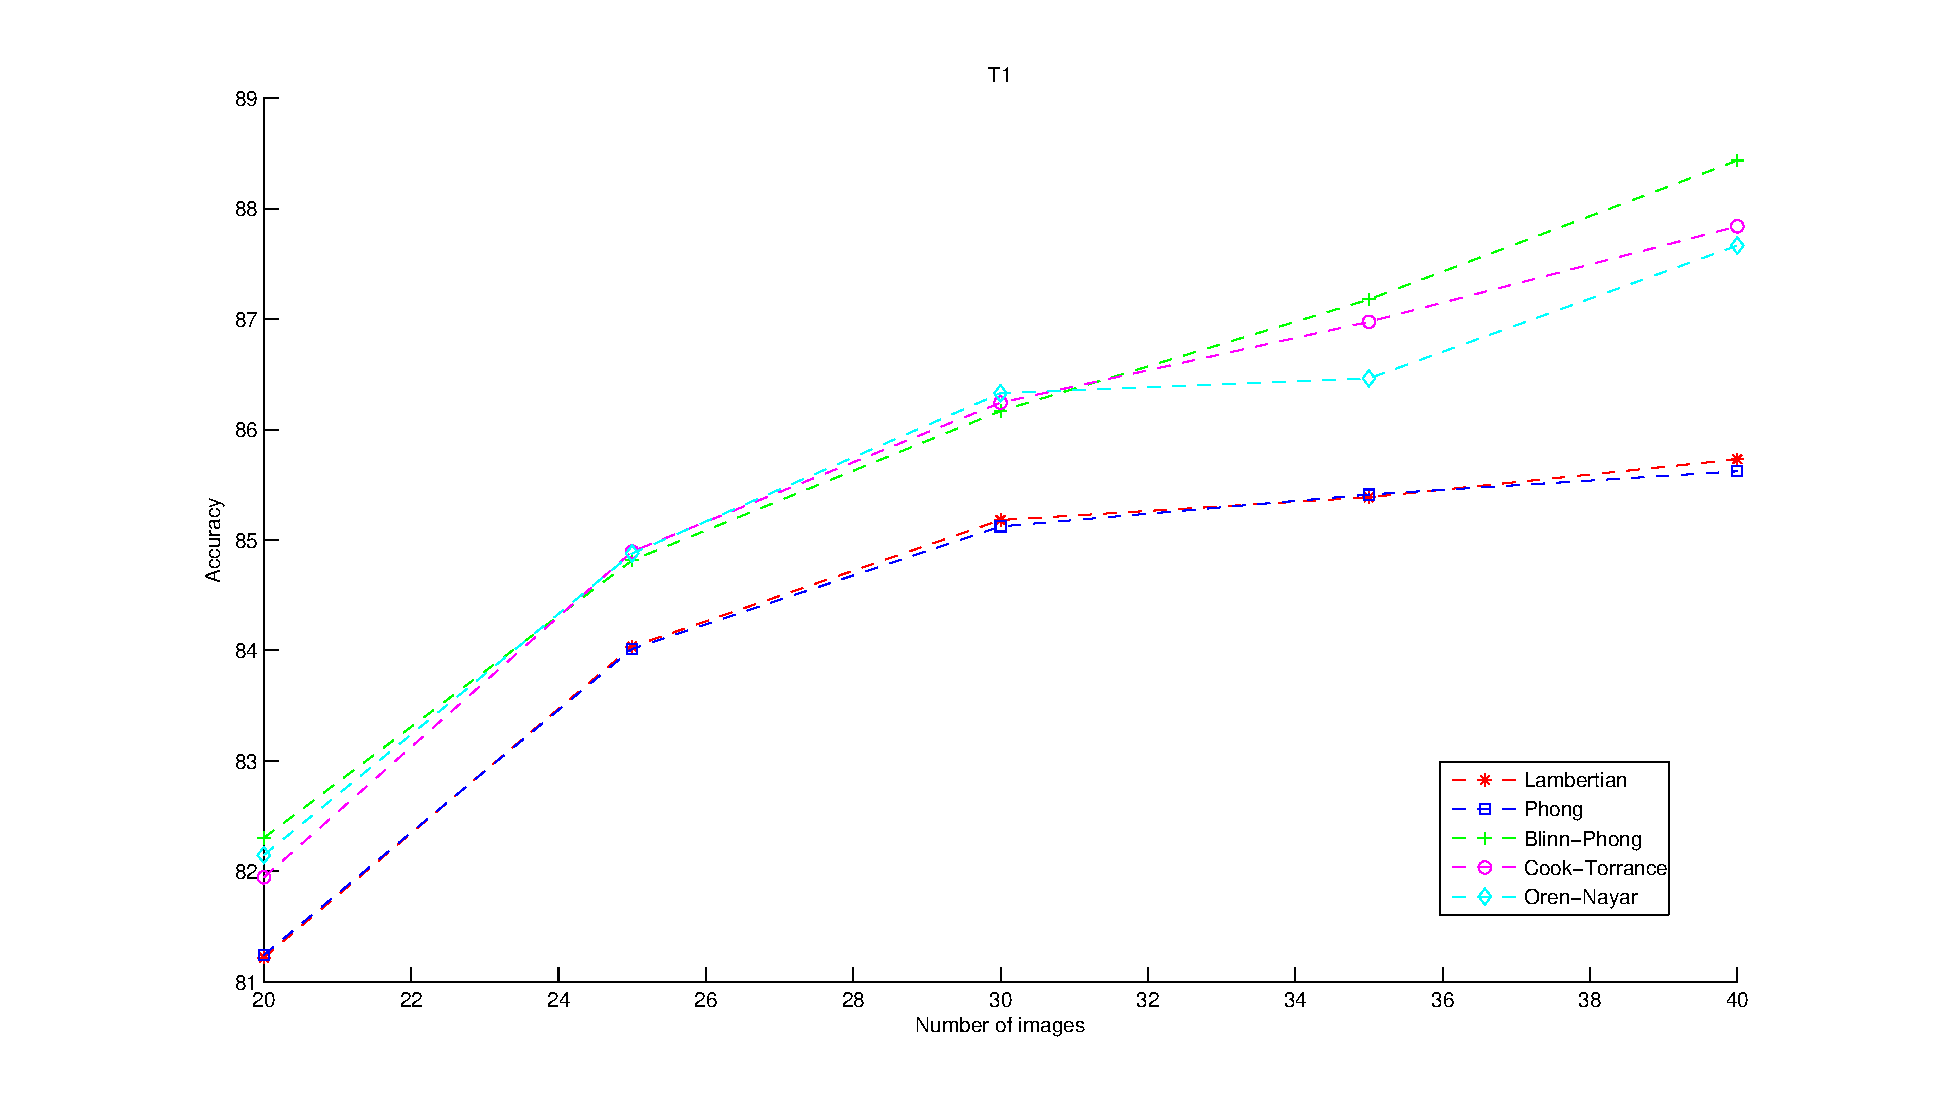
\epsfig{file=images/results/T1.eps, width=0.75\linewidth}}
		\subfigure[T3 dataset]{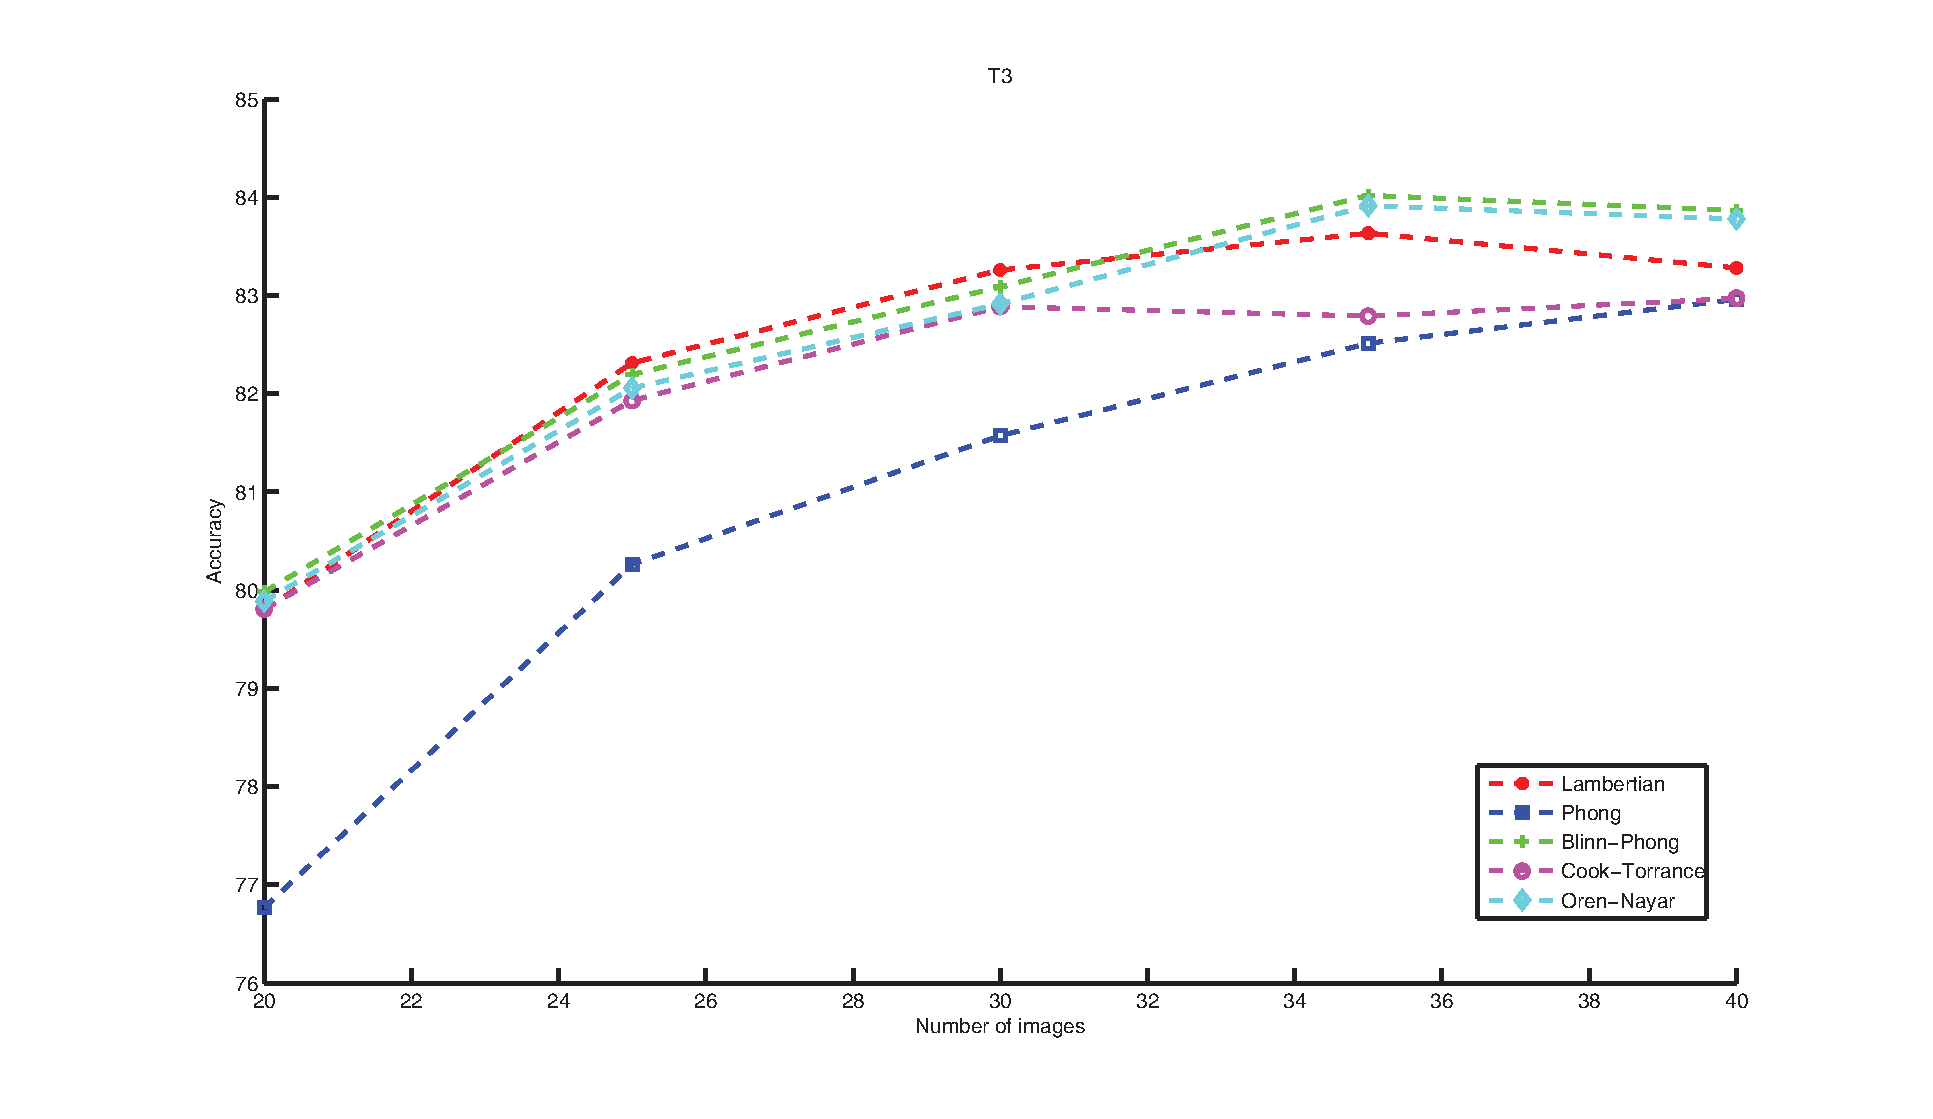
\epsfig{file=images/results/T3.eps, width=0.75\linewidth}}
		\subfigure[TT dataset]{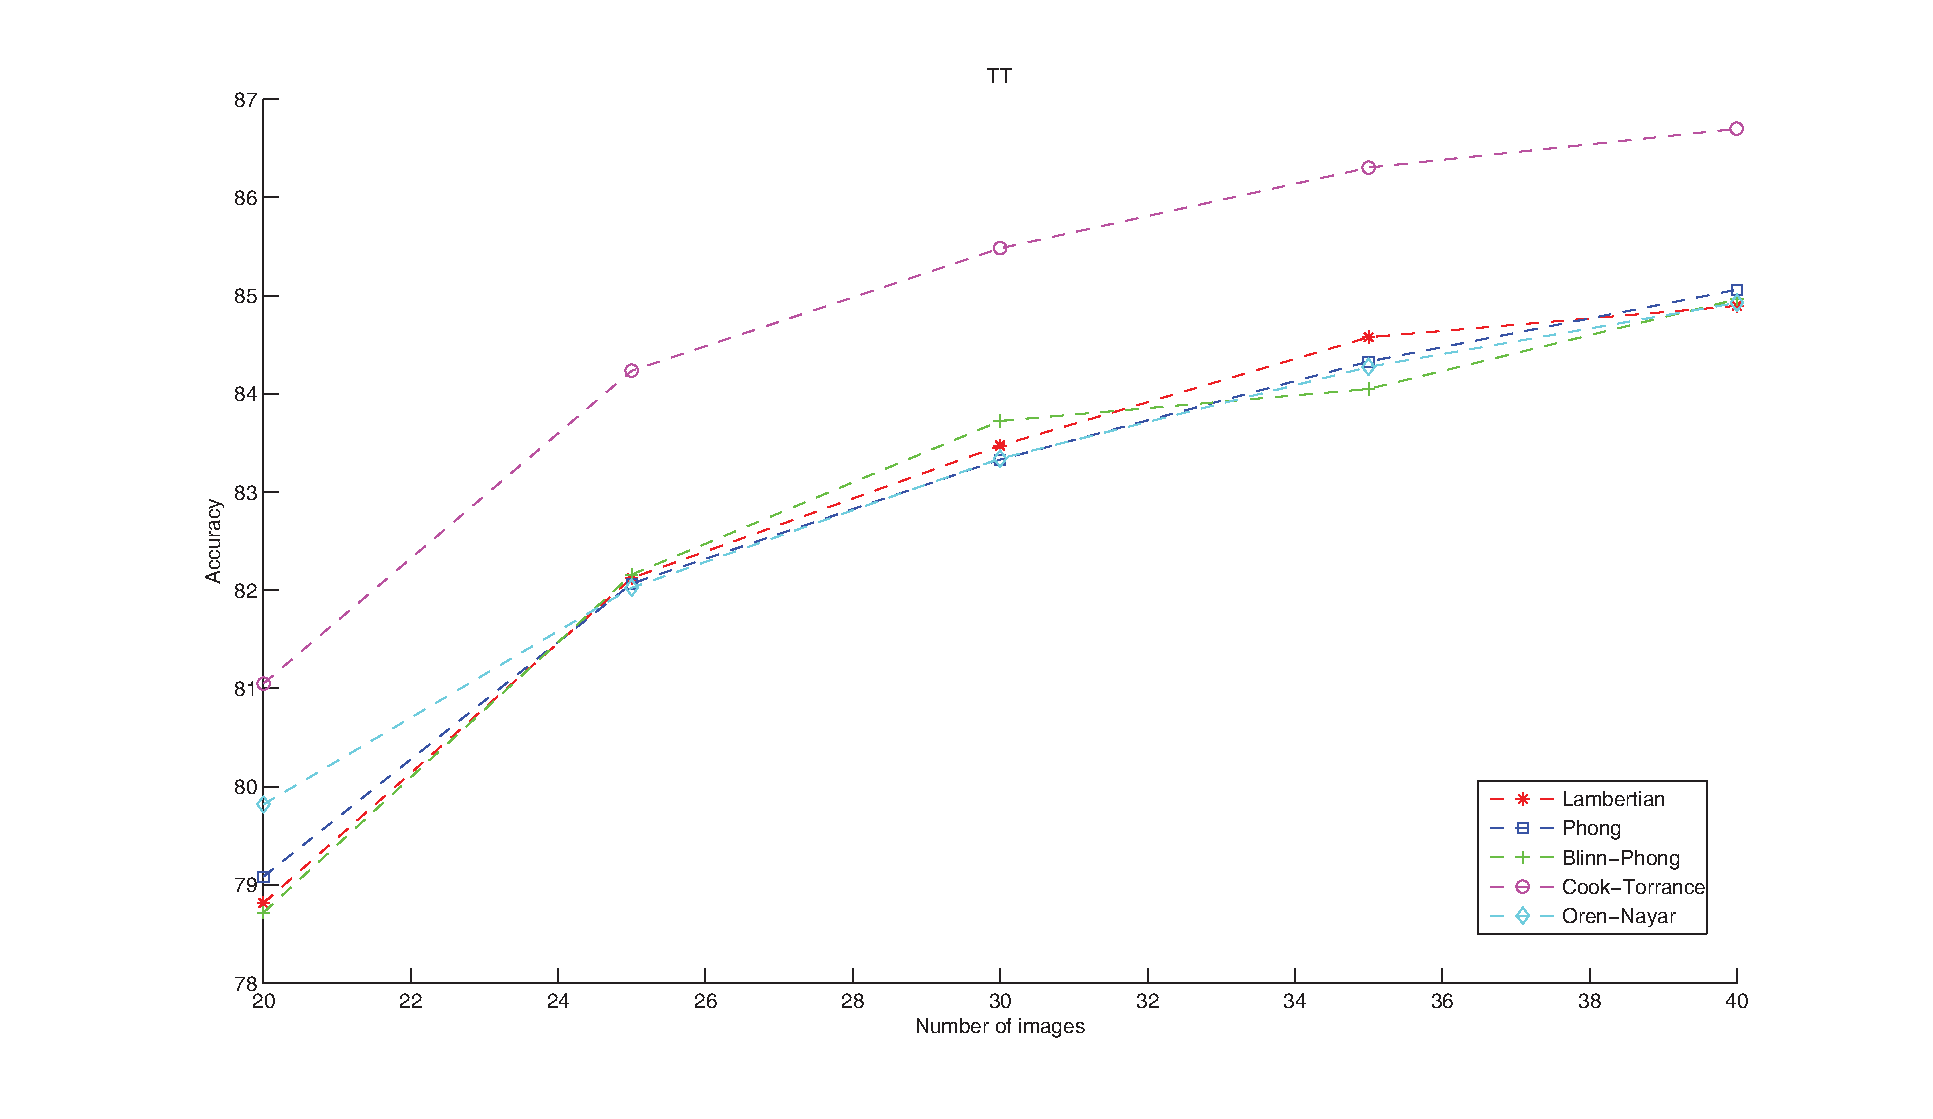
\epsfig{file=images/results/TT.eps, width=0.75\linewidth}}
	\end{center}
	\caption{{\it Results on the T1, T3 and TT dataset for diffuse materials.}}
	\label{fig:results_B}
\end{figure}


\begin{comment}

The results for experiments T1 and TT are given in figure \ref{fig:results_A}. Although the increase in accuracy compared to the Lambertian accuracy is small, figure \ref{fig:results_A}(a) clearly shows that for dataset T1 the reflectance models with physical backgrounds perform better than both Phong and Lambertian reflectance. For datasets T3 and T4 however, the accuracy drops for all reflectance models to that of the Lambertian reflectance. This can be explained, since these datasets are created by randomly picking images from T1. As a result the slant/tilt angles used for the photometric stereo procedure are not necessarily uniformly distributed, causing big errors in the photometric estimations for the surface normals and surface albedo. The resulting synthesized images are of poor quality and 

For the TT dataset, the physical reflectance models for specularity perform consistently better than Lambertian. This suggests that the addition of highlights indeed increase the quality of the synthesized images. However, it is difficult to see whether the addition of speculars on grayscale image correctly adds highlights to the material or balances out error measurements made by photometric stereo.


\begin{figure}[H]
	\begin{center}
		\subfigure[T1 dataset]{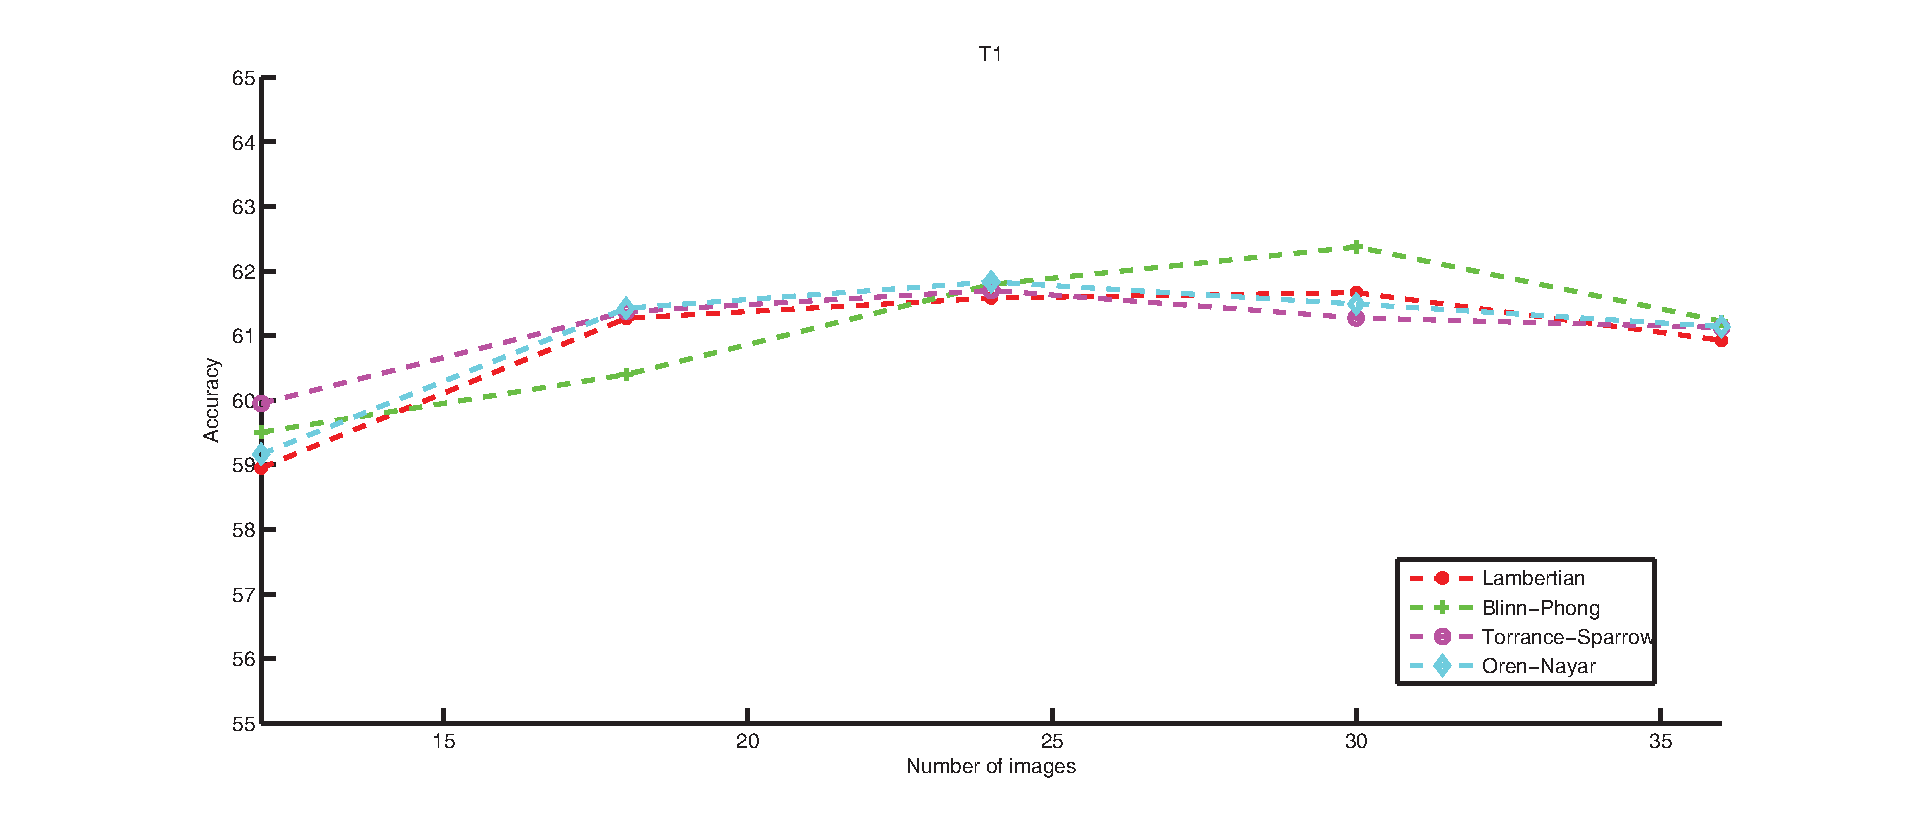
\epsfig{file=images/results/T1_specular.eps, width=0.75\linewidth}}
	\end{center}
	\caption{{\it Results on the T1 dataset for specular materials}}
	\label{fig:results_B}
\end{figure}

\end{comment}
